\scanpage{245}

donc pour $n$ grand \inserted{$(\geq n_0)$}, et $m\geq n$,
\[
\check{\mathrm H}^{*}(k'/k,M_m)\xrightarrow{\sim}\check{\mathrm H}^{*}(k'/k,M_n)
\]

\deleted{Or on a un \unsure{homomorphisme}}

\deleted{D'où facilement} Donc si $\xi_m\in\underline{\operatorname{Pic}}_{X_m/k}(k)$ est tel que son image $\xi_n$ dans $\underline{\operatorname{Pic}}_{X_n/k}(k)$ provient de $\underline{\operatorname{Pic}}(X_n)$, alors il provient lui-$=$ de $\underline{\operatorname{Pic}}(X_m)$. Ceci, et le fait que $(\underline{\operatorname{Pic}}_{X_n/k}(k))$ satisfait à M.L.(A.R.) montre que il en est de $=$ de $(\operatorname{Pic}(X_n))_n$, de façon précise si $n\geq n_0$, \deleted{\unsure{tel que il y a}} et si \deleted{\unsure{m}}\inserted{$n'$} est tel que $\operatorname{Im}(\underline{\operatorname{Pic}}_{X_{\deleted{\unsure{m}}\inserted{\unsure{n''|n'}}}/k}(k)\longrightarrow\underline{\operatorname{Pic}}_{X_n/k}(k))$ soit \unsure{minimal}, alors $\operatorname{Im}(\operatorname{Pic}(X_{\deleted{\unsure{m}}\inserted{n'}})\longrightarrow\operatorname{Pic}(X_n))$ est \unsure{minimal}. OK.

\diagram{\begin{tikzcd}[column sep=small,row sep=small]
0\arrow[r,dash] & \operatorname{Pic}(X_n)\arrow[rr,dash]\arrow[d,bend right=15] && \underline{\operatorname{Pic}}_{X_n/k}(k)\arrow[r,dash]\arrow[d,bend right=15] & \deleted{\check{\mathrm H}^2(k'/k,M_n)}\\
& \unsure{\xi_n}\arrow[rr,rightsquigarrow] && \unsure{\xi_n|\eta_n} &\\
0\arrow[r,dash] & \operatorname{Pic}(X_{n'})\arrow[uu]\arrow[rr]\arrow[d,bend right=15] && \underline{\operatorname{Pic}}_{X_{n'}/k}(k)\arrow[uu] &\\
& \xi_{n'}\arrow[uu] && &\\
0\arrow[r,dash] & \operatorname{Pic}(X_{n''})\arrow[uu]\arrow[rr,dash]\arrow[d,bend right=15] && \underline{\operatorname{Pic}}_{X_{n''}/k}(k)\arrow[uu]\arrow[d,bend right=15] &\\
& \deleted{\unsure{\xi_m}}\ \lambda_m\arrow[rr,rightsquigarrow] && \eta_m\arrow[uuuu,rightsquigarrow,bend right=25] &
\end{tikzcd}}

\uline{Corollaire} Pour que $\mathfrak X/Y$ soit \uline{projectif}, il f. et s. que pour $\forall n$, $X_n/Y_n$ \inserted{\figure{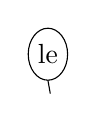
\begin{tikzpicture}[baseline=-.5ex]\draw (0,0) ellipse (.25 and .33);\node at (0,0) {le};\draw (0,-.33)--(.03,-.5);\end{tikzpicture}}} soit.

\mspage{244}
